% Created 2024-07-08 Mon 22:16
% Intended LaTeX compiler: pdflatex
\documentclass[11pt]{article}
\usepackage[utf8]{inputenc}
\usepackage[T1]{fontenc}
\usepackage{ragged2e}
\usepackage{caladea}
\usepackage{graphicx}
\usepackage{longtable}
\usepackage{wrapfig}
\usepackage{rotating}
\usepackage[normalem]{ulem}
\usepackage{hyperref}
\usepackage{amsmath}
\usepackage{amssymb}
\usepackage{capt-of}
\usepackage{hyperref}
\usepackage{fancyhdr}
\title{Novena à Santa Bibiana}
 % \hypersetup{
 %  pdfauthor={},
 %  pdftitle={Novena a/à SANTO_NOME},
 %  pdfkeywords={},
 %  pdfsubject={},
 %  pdfcreator={Emacs 29.4 (Org mode 9.6.15)}, 
 %  pdflang={English}
 % }

\title{
  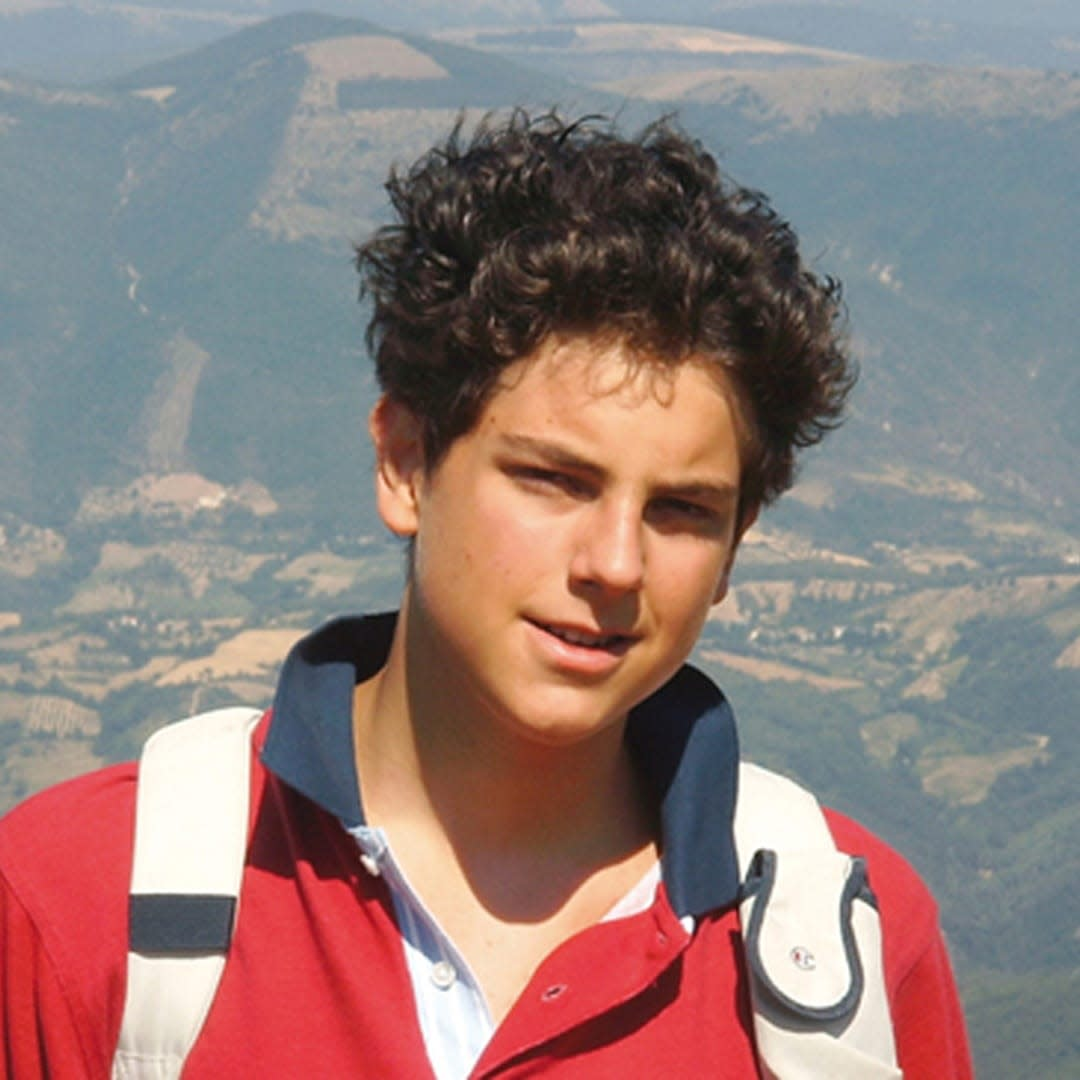
\includegraphics[scale=0.6]{./assets/imagem.jpg}
  \par
  NOVENA A SÃO NICOLAU DE MIRA}
\author{Garamog, Nina Freitas}
\date{27/11 - 05/12}
\renewcommand{\contentsname}{Sumário}

\begin{document}


\maketitle
\thispagestyle{empty}

\pagestyle{fancy}
\fancyhf{} % clear existing header/footer entries
\fancyfoot[LO, CE]{
  
\includegraphics[scale=0.2]{./assets/cross.png} São Nicolau, Rogai por Nós!
}
% Place Page X of Y on the right-hand
% side of the footer
\fancyfoot[R]{\thepage}
  
\newpage

\tableofcontents

\centering
\vfill
Visite-nos no Telegram: \url{https://t.me/CotidieNovena}
\newpage


\section{História}\label{historia}

\begin{justify}
Nicolau nasceu em Patara, uma cidadezinha marítima da Lícia, na Turquia meridional, no III século d.C., em uma família rica, que o educou ao cristianismo. A sua vida, desde a sua juventude, foi marcada pela obediência. Ao tornar-se órfão, ainda muito jovem, de pai e mãe, Nicolau, recordando a passagem evangélica do “Jovem Rico”, empregou toda a riqueza paterna à assistência dos necessitados, enfermos e pobres.

Foi nomeado Bispo de Mira e, sob o império de Diocleciano, foi exilado e preso. Depois da sua libertação, em 325, participou do Concílio de Niceia e faleceu em Mira em 343.

Foram muitos os episódios transmitidos sobre Nicolau e todos dão testemunho de uma vida ao serviço dos mais fracos, pequeninos e indefesos.

\subsection{Defensor dos fracos}

Uma das histórias mais antigas, transmitidas sobre a vida de São Nicolau, diz respeito a um seu vizinho de casa, que tinha três filhas, já na idade de se casar, mas não tinham dinheiro suficiente para comprar o dote. Para livrá-las da prostituição, certa noite, Nicolau colocou dinheiro em um pano e o jogou pela janela da casa do vizinho e saiu correndo para não ser visto. Graças àquele presente, a primogênita do vizinho conseguiu se casar. O generoso benfeitor repetiu aquele gesto, outras duas vezes, mas, na terceira noite, o pai das moças saiu rápido de casa para saber quem era aquele benfeitor. Mas o Santo lhe pediu para não dizer nada a ninguém.

Outra história diz respeito a três jovens estudantes de teologia a caminho para Atenas. O dono da hospedaria, onde os jovens tinham parado para passar a noite, os roubou e os matou, escondendo os seus corpos em uma pipa. O Bispo Nicolau, que também viajava para Atenas, parou na mesma hospedaria e, enquanto dormia, teve uma visão sobre o crime cometido pelo dono. Então, recolhendo-se em oração, São Nicolau deu novamente a vida aos três estudantes e obteve a conversão do dono malvado.

Este episódio, como o da libertação misteriosa de Basílio, - um rapaz sequestrado por piratas e vendido como doméstico a um emir, o qual, segundo a lenda, reapareceu, misteriosamente, na casa dos seus pais, com cetro de ouro do soberano estrangeiro – contribuíram para difundir a fama de Nicolau como padroeiro das crianças e dos jovens.

\subsection{Protetor dos navegantes}

Durante os anos da sua juventude, Nicolau embarcou para ir em peregrinação à Terra Santa. Passando pelos mesmos caminhos percorridos por Jesus, Nicolau rezou para poder fazer a mesma experiência, mais profunda e solidária, da vida e dos sofrimentos de Jesus. No caminho de retorno, ocorreu uma tremenda tempestade e o navio arriscava naufragar. Nicolau pôs-se, discretamente, em oração e o vento e as ondas, de repente, se acalmaram para o estupor dos marinheiros, que temiam naufragar.

\subsection{São Nicolau de Bari}

Depois da morte de São Nicolau, seu túmulo em Mira tornou logo meta de peregrinação; as suas relíquias foram consideradas milagrosas, por causa de um misterioso líquido, chamado maná de São Nicolau, que saía de dentro. Quando, no século XI, Lícia foi tomada pelos Turcos, os venezianos procuraram apoderar-se, mas foram precedidos pelos habitantes de Bari. Assim, levaram suas relíquias para a Apúlia, em 1087. Dois anos depois, foi concluída a cripta da nova igreja, desejada pelo povo de Bari, no lugar onde surgia o palácio do “catapano” bizantino. O papa Urbano II, escoltado pelos cavaleiros normandos, senhores da Apúlia, colocou as relíquias do Santo sob o altar, onde se encontram ainda hoje.

A translação das relíquias de São Nicolau teve um impacto extraordinário em toda a Europa. Na Idade Média, seu santuário na Apúlia tornou-se uma importante meta de peregrinações, com o consequente resultado da difusão do culto de São Nicolau de Bari e não com o nome de São Nicolau de Mira.

\subsection{Santa Klaus}

Nos Países Baixos, em geral, nos territórios germânicos, a festa invernal de São Nicolau (em holandês “Sint Nikolaas” e depois “Sinteklaas”) e, de modo particular, a sua proteção das crianças, deram origem à tradição infantil da espera de presentes: nas vésperas da festa do Santo, as crianças deixam sapatos ou meias sobre uma cadeira ou ao lado da lareira e vão dormir, confiantes de encontra-los no dia seguinte cheios de doces e presentes.

 

\end{justify}

\subsection*{Créditos }
\href{https://www.vaticannews.va/pt/santo-do-dia/12/06/s--nicolau-de-bari--bispo-de-mira.html}{Vatican News}

\newpage
\section{Orações}\label{oracoes}

\subsection{Oração Inicial} \label{oracao_inicial}

Deus Todo-Poderoso, Vós abençoastes São Nicolau com uma fé profunda que o ajudou a perseverar mesmo em situações difíceis. Ele defendeu corajosamente a verdade e trouxe outros até Vós pelo seu exemplo. Inspirastes São Nicolau a dar aos pobres e a servir aos que sofrem com um amor generoso e altruísta.  
Por favor, aumentai minha fé, Senhor, e ajudai-me, assim como São Nicolau, a dar generosamente àqueles que estão em necessidade, tanto em minha família quanto em minha comunidade.  
\textbf{Pai-Nosso, Avé-Maria e Glória.}

\subsection{Dia 1}

\textbf{\nameref{oracao_inicial}}

São Nicolau, você deu tudo o que tinha aos pobres sem medir esforços. Por favor, reze por aqueles que vivem na pobreza espiritual e material, para que tenham esperança em Cristo e consolação no amor de Deus. Reze também para que os membros da minha comunidade amem e sirvam os pobres, como Cristo nos ordenou.  
Por favor, ajude-me a dar livremente aos outros, a amar meu próximo e a não julgar aqueles que vivem na pobreza, mas amá-los como você fez. Ajude-me a levar a esperança de Cristo aos pobres e aos que sofrem, por meio das minhas ações e do testemunho do amor de Deus na minha vida.  
Por favor, reze também por (mencione suas intenções aqui).  

\subsection{Dia 2}

\textbf{\nameref{oracao_inicial}}

São Nicolau, você perdeu seus pais ainda jovem devido a uma doença. Por favor, reze pelas crianças que não têm pais amorosos, para que sejam consoladas pela paz de Cristo. Por favor, ajude-me a amar e aprender com as crianças da minha vida, para que eu possa emular sua fé simples e seu encanto pelo mundo.  
Reze por mim, para que eu ame a Deus com uma fé de criança, confiando completamente nele, mesmo em meio ao sofrimento e à perda. Ajude-me a lembrar que Deus é um bom Pai e sabe o que é melhor para mim, mesmo quando eu não compreendo.  
Por favor, reze também por (mencione suas intenções aqui).  

\vfill

\subsection{Dia 3}

\textbf{\nameref{oracao_inicial}}

São Nicolau, como sacerdote e bispo, você testemunhou muitos casamentos sacramentais e preparou noivos para o Sacramento do Matrimônio. Por favor, reze por aqueles que são casados ou estão se preparando para o casamento, para que busquem sempre amar um ao outro de forma livre, total, fiel e frutífera.  
Reze por mim, para que eu viva fielmente a vocação para a qual Deus me chamou ou está me chamando. Ajude-me a amar meu (cônjuge/família) e a buscar formas de carregar minha cruz e seguir o Senhor na minha vocação a cada dia.  
Por favor, reze também por (mencione suas intenções aqui).  

\subsection{Dia 4}

\textbf{\nameref{oracao_inicial}}

São Nicolau, sua generosidade e respeito pela dignidade humana salvaram três mulheres de uma vida de prostituição. Por favor, reze por adultos e crianças presos em situações de tráfico humano ou prostituição, para que sejam libertos dessas circunstâncias e conheçam o amor de Deus em suas vidas.  
Reze por mim, para que eu veja e honre a dignidade de cada pessoa humana que encontro e defenda a dignidade humana sempre que tiver a oportunidade.  
Por favor, reze também por (mencione suas intenções aqui).  

\subsection{Dia 5}

\textbf{\nameref{oracao_inicial}}

São Nicolau, você experimentou a dor de perder seus pais ainda jovem. No entanto, transformou essa perda em algo belo e santo, usando sua herança para servir aos pobres e aos que sofriam na sua comunidade.  
Por favor, interceda por aqueles que perderam seus pais, para que sejam confortados pela paz de Cristo e consolados. Reze por mim, para que eu confie em Deus e em Seu plano para minha vida, mesmo nos momentos de perda e luto.  
Por favor, reze também por (mencione suas intenções aqui).  

\vfill
\subsection{Dia 6}

\textbf{\nameref{oracao_inicial}}

São Nicolau, você levou a sério seu papel de guardião do depósito da fé, mesmo sendo perseguido por sua devoção à Igreja. Por favor, reze por todos aqueles que ensinam a fé, para que o façam com eloquência e fidelidade, ensinando os fiéis sobre Jesus e a Igreja que Ele estabeleceu.  
Reze por mim, para que eu aprenda continuamente mais sobre Jesus Cristo e os ensinamentos da Igreja, crescendo no conhecimento de Cristo e de Seu amor por mim.  
Por favor, reze também por (mencione suas intenções aqui).  

\subsection{Dia 7}

\textbf{\nameref{oracao_inicial}}

São Nicolau, sua piedade e humildade levaram-no a se tornar o bispo de Mira. Você defendeu a fé contra a heresia ariana e foi um exemplo santo de fé e caridade cristãs para os fiéis que serviu. Por favor, reze pelo meu bispo (insira o nome do bispo aqui), para que ele seja um servo fiel de Cristo, mesmo em meio a provas e perseguições.  
Reze por todos os sacerdotes e membros do clero, para que sejam encorajados na fé e motivados a trazer almas para Cristo, mesmo quando isso for difícil ou desconfortável.  
Por favor, reze também por (mencione suas intenções aqui).  

\subsection{Dia 8}

\textbf{\nameref{oracao_inicial}}

São Nicolau, você viveu corajosamente como cristão durante o reinado de Diocleciano, quando o Cristianismo era severamente perseguido. Você suportou tortura, prisão e encarceramento por praticar sua fé. Reze por aqueles que são igualmente perseguidos, para que sejam consolados pela presença e promessas de Deus e permaneçam firmes em viver sua fé cristã.  
Reze por mim, para que eu tenha coragem de praticar minha fé, mesmo em situações em que possa ser perseguido ou me sentir desconfortável.  
Por favor, reze também por (mencione suas intenções aqui).  

\vfill
\subsection{Dia 9}

\textbf{\nameref{oracao_inicial}}

São Nicolau, sua vida e testemunho de Cristo nos ensinam a seguir as palavras de Cristo: amar e servir os pobres, a qualquer custo, e viver corajosamente nossa fé, mesmo diante da perseguição. Reze por mim, para que eu viva minha fé com a mesma ousadia que você viveu.  
Por favor, interceda por mim, para que minha fé em Cristo aumente e minha confiança no Senhor acalme meus medos sobre as incertezas do futuro.  
Por favor, reze também por (mencione suas intenções aqui).  


\subsection*{Créditos:}
\href{https://www.praymorenovenas.com/st-nicholas-novena}{ Pray More Novenas}


\end{document}
